\documentclass{standalone}
\usepackage{tikz}
\usetikzlibrary{patterns, positioning}


\begin{document}
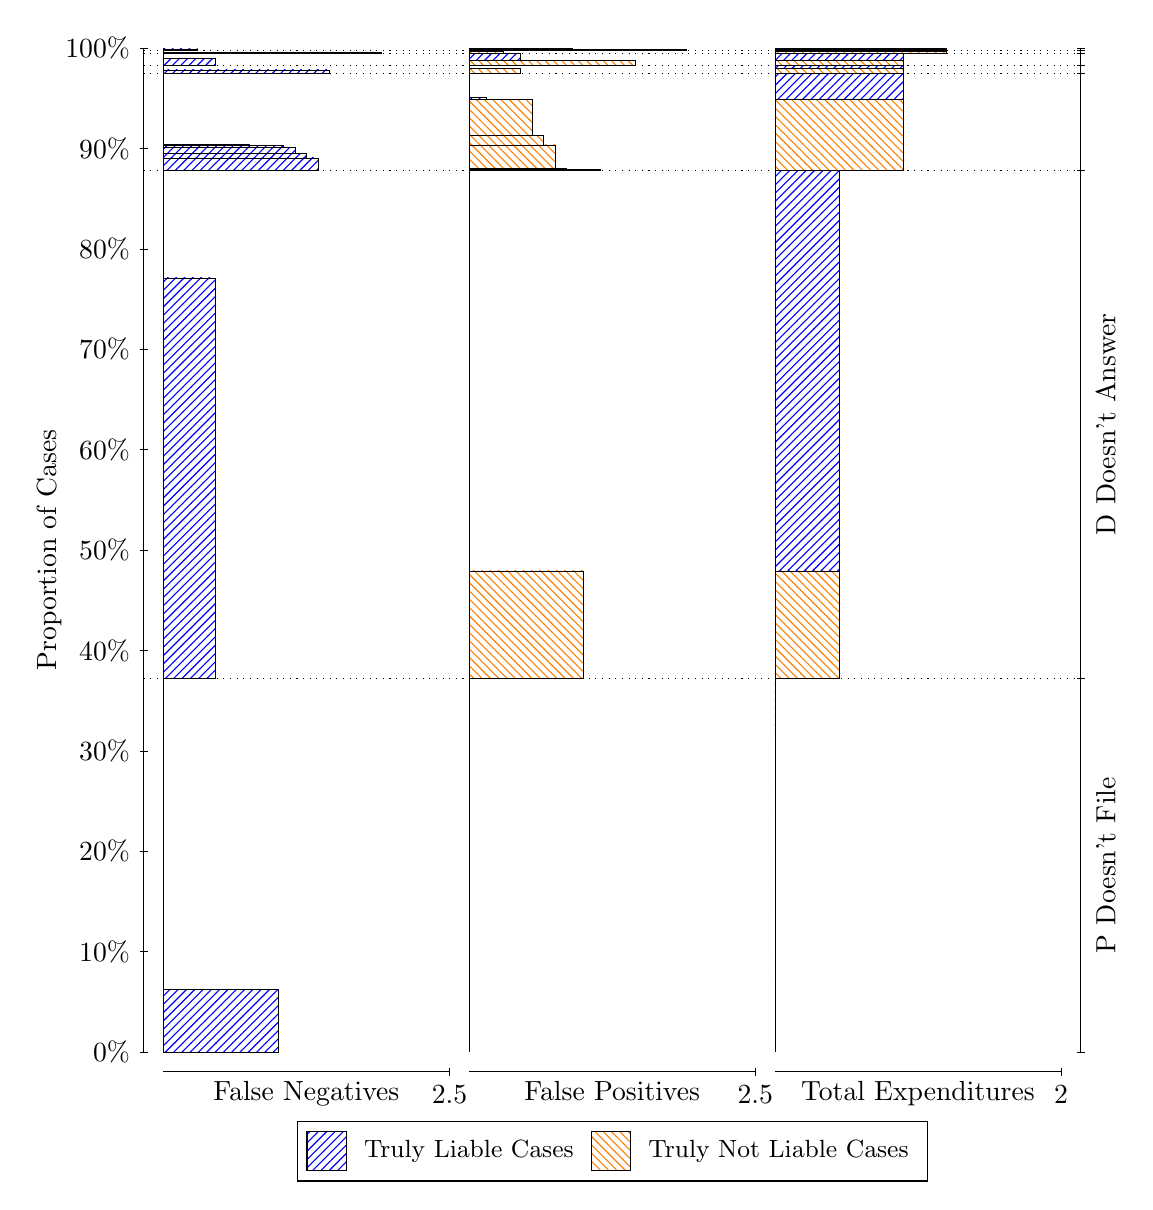
\begin{tikzpicture}
\draw[black, very thin] (1.5,1.75) -- (1.5,14.5);
\node[rotate=90, text=black, anchor=center] at (0.3, 8.125) {Proportion of Cases};
\draw[black, very thin] (1.45,1.75) -- (1.55,1.75);
\node[text=black, anchor=east] at (1.45, 1.75) {0\%};
\draw[black, very thin] (1.45,3.025) -- (1.55,3.025);
\node[text=black, anchor=east] at (1.45, 3.025) {10\%};
\draw[black, very thin] (1.45,4.3) -- (1.55,4.3);
\node[text=black, anchor=east] at (1.45, 4.3) {20\%};
\draw[black, very thin] (1.45,5.575) -- (1.55,5.575);
\node[text=black, anchor=east] at (1.45, 5.575) {30\%};
\draw[black, very thin] (1.45,6.85) -- (1.55,6.85);
\node[text=black, anchor=east] at (1.45, 6.85) {40\%};
\draw[black, very thin] (1.45,8.125) -- (1.55,8.125);
\node[text=black, anchor=east] at (1.45, 8.125) {50\%};
\draw[black, very thin] (1.45,9.4) -- (1.55,9.4);
\node[text=black, anchor=east] at (1.45, 9.4) {60\%};
\draw[black, very thin] (1.45,10.675) -- (1.55,10.675);
\node[text=black, anchor=east] at (1.45, 10.675) {70\%};
\draw[black, very thin] (1.45,11.95) -- (1.55,11.95);
\node[text=black, anchor=east] at (1.45, 11.95) {80\%};
\draw[black, very thin] (1.45,13.225) -- (1.55,13.225);
\node[text=black, anchor=east] at (1.45, 13.225) {90\%};
\draw[black, very thin] (1.45,14.5) -- (1.55,14.5);
\node[text=black, anchor=east] at (1.45, 14.5) {100\%};

\draw[black, very thin] (13.4,1.75) -- (13.4,14.5);
\draw[black, very thin] (13.35,1.75) -- (13.45,1.75);
\node[anchor=west] at (13.35, 1.75) {};
\draw[black, very thin] (13.35,6.4945) -- (13.45,6.4945);
\node[anchor=west] at (13.35, 6.4945) {};
\draw[black, very thin] (13.35,12.949) -- (13.45,12.949);
\node[anchor=west] at (13.35, 12.949) {};
\draw[black, very thin] (13.35,14.18) -- (13.45,14.18);
\node[anchor=west] at (13.35, 14.18) {};
\draw[black, very thin] (13.35,14.279) -- (13.45,14.279);
\node[anchor=west] at (13.35, 14.279) {};
\draw[black, very thin] (13.35,14.428) -- (13.45,14.428);
\node[anchor=west] at (13.35, 14.428) {};
\draw[black, very thin] (13.35,14.466) -- (13.45,14.466);
\node[anchor=west] at (13.35, 14.466) {};
\draw[black, very thin] (13.35,14.5) -- (13.45,14.5);
\node[anchor=west] at (13.35, 14.5) {};

\draw[black, very thin, pattern color=blue, pattern=north east lines] (1.75,1.75) rectangle (3.2033,2.5477);
\draw[black, very thin, pattern color=orange, pattern=north west lines] (1.75,2.5477) rectangle (1.75,6.4945);
\draw[black, very thin, pattern color=blue, pattern=north east lines] (1.75,6.4945) rectangle (2.404,11.582);
\draw[black, very thin, pattern color=orange, pattern=north west lines] (1.75,11.582) rectangle (1.75,12.949);
\draw[black, very thin, pattern color=blue, pattern=north east lines] (1.75,12.949) rectangle (3.712,13.105);
\draw[black, very thin, pattern color=blue, pattern=north east lines] (1.75,13.105) rectangle (3.5667,13.163);
\draw[black, very thin, pattern color=blue, pattern=north east lines] (1.75,13.163) rectangle (3.4213,13.241);
\draw[black, very thin, pattern color=blue, pattern=north east lines] (1.75,13.241) rectangle (3.276,13.259);
\draw[black, very thin, pattern color=blue, pattern=north east lines] (1.75,13.259) rectangle (3.1307,13.26);
\draw[black, very thin, pattern color=blue, pattern=north east lines] (1.75,13.26) rectangle (2.84,13.278);
\draw[black, very thin, pattern color=orange, pattern=north west lines] (1.75,13.278) rectangle (1.75,14.18);
\draw[black, very thin, pattern color=blue, pattern=north east lines] (1.75,14.18) rectangle (3.8573,14.221);
\draw[black, very thin, pattern color=orange, pattern=north west lines] (1.75,14.221) rectangle (1.75,14.279);
\draw[black, very thin, pattern color=blue, pattern=north east lines] (1.75,14.279) rectangle (2.404,14.365);
\draw[black, very thin, pattern color=orange, pattern=north west lines] (1.75,14.365) rectangle (1.75,14.428);
\draw[black, very thin, pattern color=blue, pattern=north east lines] (1.75,14.428) rectangle (4.5113,14.44);
\draw[black, very thin, pattern color=orange, pattern=north west lines] (1.75,14.44) rectangle (1.75,14.466);
\draw[black, very thin, pattern color=blue, pattern=north east lines] (1.75,14.466) rectangle (2.186,14.488);
\draw[black, very thin, pattern color=orange, pattern=north west lines] (1.75,14.488) rectangle (1.75,14.5);
\draw[black, very thin, pattern color=orange, pattern=north west lines] (5.6333,1.75) rectangle (5.6333,5.6968);
\draw[black, very thin, pattern color=blue, pattern=north east lines] (5.6333,5.6968) rectangle (5.6333,6.4945);
\draw[black, very thin, pattern color=orange, pattern=north west lines] (5.6333,6.4945) rectangle (7.0867,7.8611);
\draw[black, very thin, pattern color=blue, pattern=north east lines] (5.6333,7.8611) rectangle (5.6333,12.949);
\draw[black, very thin, pattern color=orange, pattern=north west lines] (5.6333,12.949) rectangle (7.3047,12.956);
\draw[black, very thin, pattern color=orange, pattern=north west lines] (5.6333,12.956) rectangle (7.014,12.956);
\draw[black, very thin, pattern color=orange, pattern=north west lines] (5.6333,12.956) rectangle (6.8687,12.975);
\draw[black, very thin, pattern color=orange, pattern=north west lines] (5.6333,12.975) rectangle (6.7233,13.269);
\draw[black, very thin, pattern color=orange, pattern=north west lines] (5.6333,13.269) rectangle (6.578,13.395);
\draw[black, very thin, pattern color=orange, pattern=north west lines] (5.6333,13.395) rectangle (6.4327,13.851);
\draw[black, very thin, pattern color=blue, pattern=north east lines] (5.6333,13.851) rectangle (5.8513,13.869);
\draw[black, very thin, pattern color=blue, pattern=north east lines] (5.6333,13.869) rectangle (5.6333,14.18);
\draw[black, very thin, pattern color=orange, pattern=north west lines] (5.6333,14.18) rectangle (6.2873,14.238);
\draw[black, very thin, pattern color=blue, pattern=north east lines] (5.6333,14.238) rectangle (5.6333,14.279);
\draw[black, very thin, pattern color=orange, pattern=north west lines] (5.6333,14.279) rectangle (7.7407,14.343);
\draw[black, very thin, pattern color=blue, pattern=north east lines] (5.6333,14.343) rectangle (6.2873,14.428);
\draw[black, very thin, pattern color=orange, pattern=north west lines] (5.6333,14.428) rectangle (6.0693,14.454);
\draw[black, very thin, pattern color=blue, pattern=north east lines] (5.6333,14.454) rectangle (5.6333,14.466);
\draw[black, very thin, pattern color=orange, pattern=north west lines] (5.6333,14.466) rectangle (8.3947,14.478);
\draw[black, very thin, pattern color=blue, pattern=north east lines] (5.6333,14.478) rectangle (6.9413,14.5);
\draw[black, very thin, pattern color=orange, pattern=north west lines] (9.5167,1.75) rectangle (9.5167,5.6968);
\draw[black, very thin, pattern color=blue, pattern=north east lines] (9.5167,5.6968) rectangle (9.5167,6.4945);
\draw[black, very thin, pattern color=orange, pattern=north west lines] (9.5167,6.4945) rectangle (10.334,7.8611);
\draw[black, very thin, pattern color=blue, pattern=north east lines] (9.5167,7.8611) rectangle (10.334,12.949);
\draw[black, very thin, pattern color=orange, pattern=north west lines] (9.5167,12.949) rectangle (11.152,13.851);
\draw[black, very thin, pattern color=blue, pattern=north east lines] (9.5167,13.851) rectangle (11.152,14.18);
\draw[black, very thin, pattern color=orange, pattern=north west lines] (9.5167,14.18) rectangle (11.152,14.238);
\draw[black, very thin, pattern color=blue, pattern=north east lines] (9.5167,14.238) rectangle (11.152,14.279);
\draw[black, very thin, pattern color=orange, pattern=north west lines] (9.5167,14.279) rectangle (11.152,14.343);
\draw[black, very thin, pattern color=blue, pattern=north east lines] (9.5167,14.343) rectangle (11.152,14.428);
\draw[black, very thin, pattern color=orange, pattern=north west lines] (9.5167,14.428) rectangle (11.697,14.454);
\draw[black, very thin, pattern color=blue, pattern=north east lines] (9.5167,14.454) rectangle (11.697,14.466);
\draw[black, very thin, pattern color=orange, pattern=north west lines] (9.5167,14.466) rectangle (11.697,14.478);
\draw[black, very thin, pattern color=blue, pattern=north east lines] (9.5167,14.478) rectangle (11.697,14.5);
\draw[black, dotted] (1.5,6.4945) -- (13.4,6.4945);
\draw[black, dotted] (1.5,12.949) -- (13.4,12.949);
\draw[black, dotted] (1.5,14.18) -- (13.4,14.18);
\draw[black, dotted] (1.5,14.279) -- (13.4,14.279);
\draw[black, dotted] (1.5,14.428) -- (13.4,14.428);
\draw[black, dotted] (1.5,14.466) -- (13.4,14.466);
\draw[black, very thin] (1.75,1.5) -- (5.3833,1.5);
\node[text=black, anchor=north] at (3.5667, 1.5) {False Negatives};
\draw[black, very thin] (5.3833,1.45) -- (5.3833,1.55);
\node[text=black, anchor=north] at (5.3833, 1.45) {2.5};

\draw[black, very thin] (5.6333,1.5) -- (9.2667,1.5);
\node[text=black, anchor=north] at (7.45, 1.5) {False Positives};
\draw[black, very thin] (9.2667,1.45) -- (9.2667,1.55);
\node[text=black, anchor=north] at (9.2667, 1.45) {2.5};

\draw[black, very thin] (9.5167,1.5) -- (13.15,1.5);
\node[text=black, anchor=north] at (11.333, 1.5) {Total Expenditures};
\draw[black, very thin] (13.15,1.45) -- (13.15,1.55);
\node[text=black, anchor=north] at (13.15, 1.45) {2};

\node[text=black, centered, rotate=90] at (13.72, 4.1223) {P Doesn't File};
\node[text=black, centered, rotate=90] at (13.72, 9.7218) {D Doesn't Answer};






\draw (7.449999999999999,1.5) node[draw=none] (baseCoordinate) {};
\begin{scope}[align=center]
        \matrix[scale=0.5, draw=black, below=0.5cm of baseCoordinate, nodes={draw}, column sep=0.1cm]{
            \node[rectangle, draw, minimum width=0.5cm, minimum height=0.5cm, pattern color=blue, pattern=north east lines] {}; &
            \node[draw=none, font=\small, text=black] (B) {Truly Liable Cases}; &
            \node[rectangle, draw, minimum width=0.5cm, minimum height=0.5cm, pattern color=orange, pattern=north west lines] {}; &
            \node[draw=none, font=\small, text=black] (B) {Truly Not Liable Cases}; \\
            };
\end{scope}

\end{tikzpicture}
\end{document}